% v0.1
\chapter{Bacteriophages}
In this chapter we will provide detailed description of bacteriophages, which will be the central topic of our work.
We will describe what they are and where we can find them.
We will also show currently valid taxonomical classification and the structure of a typical representative of this group of organisms.
Furthermore, we will explain their life cycle and we will point out some of their use.
% At the end of this chapter we will point out what was already done in this field and what we would like to achieve.

\section{Origin of bacteriophages}
\emph{Bacteriophages} (phages) belong to the group of viruses, which have the capability to infect and replicate within bacterial hosts.
It is estimated that they are the most abundant group of entities on Earth with their estimated count around $10^{31}$\cite{phage}.
In comparison, it is estimated that the count of all bacteria on planet Earth is around $10^{30}$.
They are one of the most highly diverse group in the biosphere, with their genomes spanning from few genes to as many as hundreds of genes.
We can find them in every place on earth, where bacteria are able to live, even inside our bodies.
It is believed that one of the most saturated location of their occurrence is sea, with  $9\cdot 10^8$ virions per milliliter of seawater at the surface and 70\% of bacteria infected \cite{virioplankton}.
Thanks to the high abundance of bacteriophages, their impact on shaping of the environment is outstandingly significant.
% + circulating carbon?
% + they contribute to horizontal gene transfer via transduction and transformation

\section{Taxonomical classification}
Classification of bacteriophages is difficult mainly due to their high diversity and genome mosaicism. \cite{phagetax}
Consequently, there exists no universal marker similar to 16S rRNA gene in bacteria, according to which we will be able to classify bacteriophages based on their genetic information.
This is because no genes are strongly conserved within all bacteriophages.
Despite of these facts, there is taxonomical classification of phages.
This classification was created by International Committee on Taxonomy of Viruses (ICTV) and it categorizes each phage according to its morphology and nucleic acid.
This taxonomy recognizes nineteen different families of phages.
Although this taxonomy is currently in use, many biologists feel it is outdated and in need of revision. \cite{phagetax}

\section{Structure of a typical bacteriophage}
Given the high variety of bacteriophages, they come in a lot of different sizes and shapes.
Each bacteriophage consists of genetic information in form of DNA or RNA and capsid, a protein coat usually composited from higher number of identical protein units.
We will describe the most typical form of bacteriophages, which is abundantly found in nature.

\begin{figure}[h]
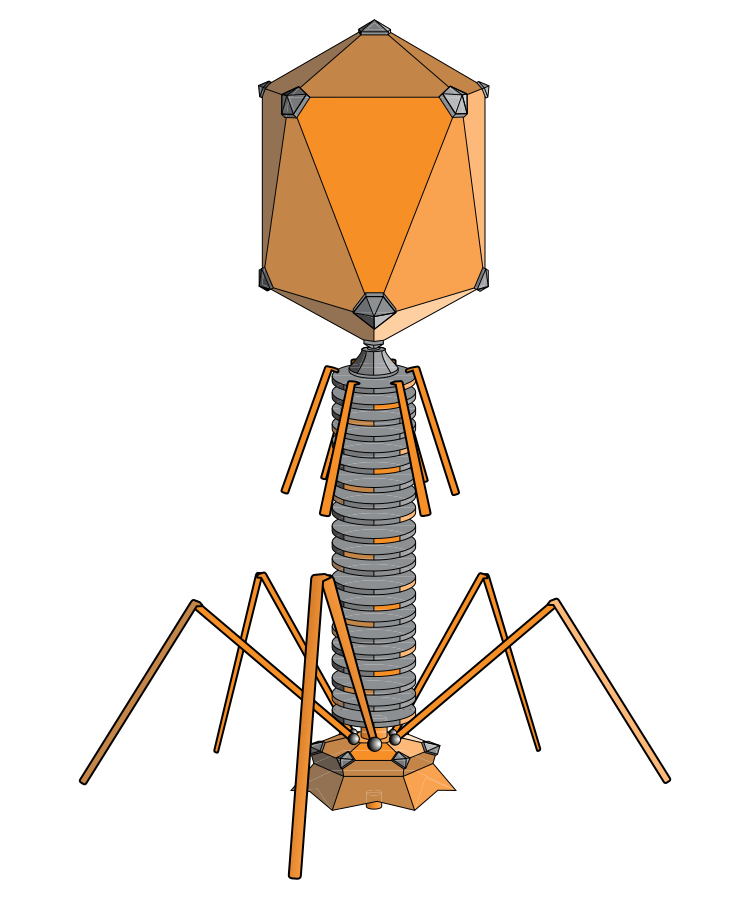
\includegraphics[width=0.5\textwidth]{./images/phage.png}
\centering
\caption{Structure of a typical bacteriophage
%By Adenosine [CC BY-SA 3.0 (https://creativecommons.org/licenses/by-sa/3.0) or GFDL (http://www.gnu.org/copyleft/fdl.html)], from Wikimedia Commons
}
\label{fig:phage}
\end{figure}


As we can see in the Figure \ref{fig:phage}, this bacteriophages body consists of a head and a tail.
These parts are created from proteins and in addition, the head contains DNA or RNA of the bacteriophage genome.
The tail is used to attach and to inject the genetic code into bacteria.
At the end of the tail, there are proteins, which are able to bind to specific receptors on the surface of a bacteria.
Thanks to this mechanism, bacteriophages tend to have a high specificity in selection of their prey.

\section{Life cycle of bacteriophages}
Generally, there are two strategies that bacteriophages use to secure their survival and replication; the \emph{lysogenic cycle} and the \emph{lytic cycle}.
Viruses tend to use these strategies in different proportions, but usually prefer to choose one of them.
The lysogenic cycle results in incorporations of phage genetic information into host DNA or creation of a circular replicon in the bacterial cytoplasm.
By this approach, the genetic material of a phage inside the host, called prophage, is duplicated together with the host genome and after cell division, both daughter cells contain DNA of the bacteriophage.
In dependence on the following events, viral DNA can be released from hosts genome and start proliferation of new phages via the lytic cycle.
The lytic cycle is characterized by the lysis of bacterial cells membrane and their subsequent death.
It starts by injecting bacteriophage genome into bacteria.
After this step virus is not incorporated, but it compromises bacterial translation apparatus to produce more viruses.
Once enough virions have been produced, special viral proteins dissolve the bacterial cell and virions are released into surrounding space.

\section{Potential usage of bacteriophages}
Their ability to kill or alter behavior of highly specific strains of bacteria makes bacteriophages a valuable target for research.
Humankind tried to harness the power of phages since their discovery in the year 1917.
This discovery is attributed to a French-Canadian microbiologist Félix d'Hérelle, who experimented extensively with phages and introduced the concept of \emph{phage therapy}\cite{phages_in_nature}.
Unfortunately, after the discovery of antibiotics, research in this field suffered from insufficient funding and the development was significantly slowed down.\\
Nowadays, when humanity face the threat of multiresistant bacteria and phages could bring a new methods into the battle against pathogenic bacteria, the research in this field begins to flourish.
We can see the potential of their use in the field of food industry as the substances that are prolonging life and improve the quality of our food. In the field of pharmacy, they are used as medicines for bacterial infections. Their use is significant when we encounter the need to control the lives of microbial communities.
Moreover, due to their high specificity to a particular strain of bacteria, these new practices will likely be without adverse effects on natural microbiome.

% \section{Phage effectiveness}
% documented case of use from india
% georgia - cocktails
% bacterial mechanisms to prevent

\section{Current state of knowledge}
In our work we focus on prediction of phage hosts from genomic sequence.
We based our method on the assumption that bacteriophages with similar set of genes will infect the same bacterial host.
In addition, the decision to pick the host as our trait of interest was made based on its straightforward use in searching for phages suitable for phage therapy.
Attempts to classify bacteriophages from a genomic sequence were already made.
In the study "The Phage Proteomic Tree: a Genome-Based Taxonomy for Phage"\cite{phage} from year 2002, researchers performed analysis based on genomes resulting in phylogenetic tree compatible with ICTV system.
In their work, they proved phages indeed do not contain any universal genetic marker, which could be used as 16S rRNA sequence for classification.
They also showed that classification based on whole proteome of phage is a reasonable approach.
In 2016 a similar tool, called HostPhinder, for predicting hosts from genomic sequences appeared \cite{hostphinder}.
Their approach to classification was through rate of similar k-mers, short sequences of nucleotides of length $k$.
With this approach they achieved the results of 81\% of correctly predicted genera.
In our work we tried a different approach, where we looked for similar genes instead of rate of similar k-mers.  

% +https://academic.oup.com/bioinformatics/article/33/19/3113/3964377
% +virhostmatcher
